\documentclass{../source/Experiment}

\major{信息工程}
\name{姚桂涛}
\title{局部保持映射(LPP)}
\stuid{3190105597}
\college{信息与电子工程学院}
\date{\today}
\lab{教11-400}
\course{人工智能实验}
\instructor{胡浩基、魏准}
\grades{}
\expname{局部保持映射(LPP)}
\exptype{设计验证}
\partner{}
\begin{document}
    \makecover
    \section{实验题目}
        \subsection{实验4-4}
        利用sklearn.datasets.load\_digits函数,导入手写数字数据集作为푋푇,通过LPP对生成的随机数据进行降维(n\_dim=2),并可视化降维后的数据。

    \section{实验代码}
    \subsection{LPP.py}
    \lstinputlisting[
        language  =   Python,
        title = {LPP.py}
        ]{./Part4/4-4.py}
   

    \section{实验结果}
        \subsection{实验4-4}
            可视化结果
            \begin{figure}[H]
                \centering
                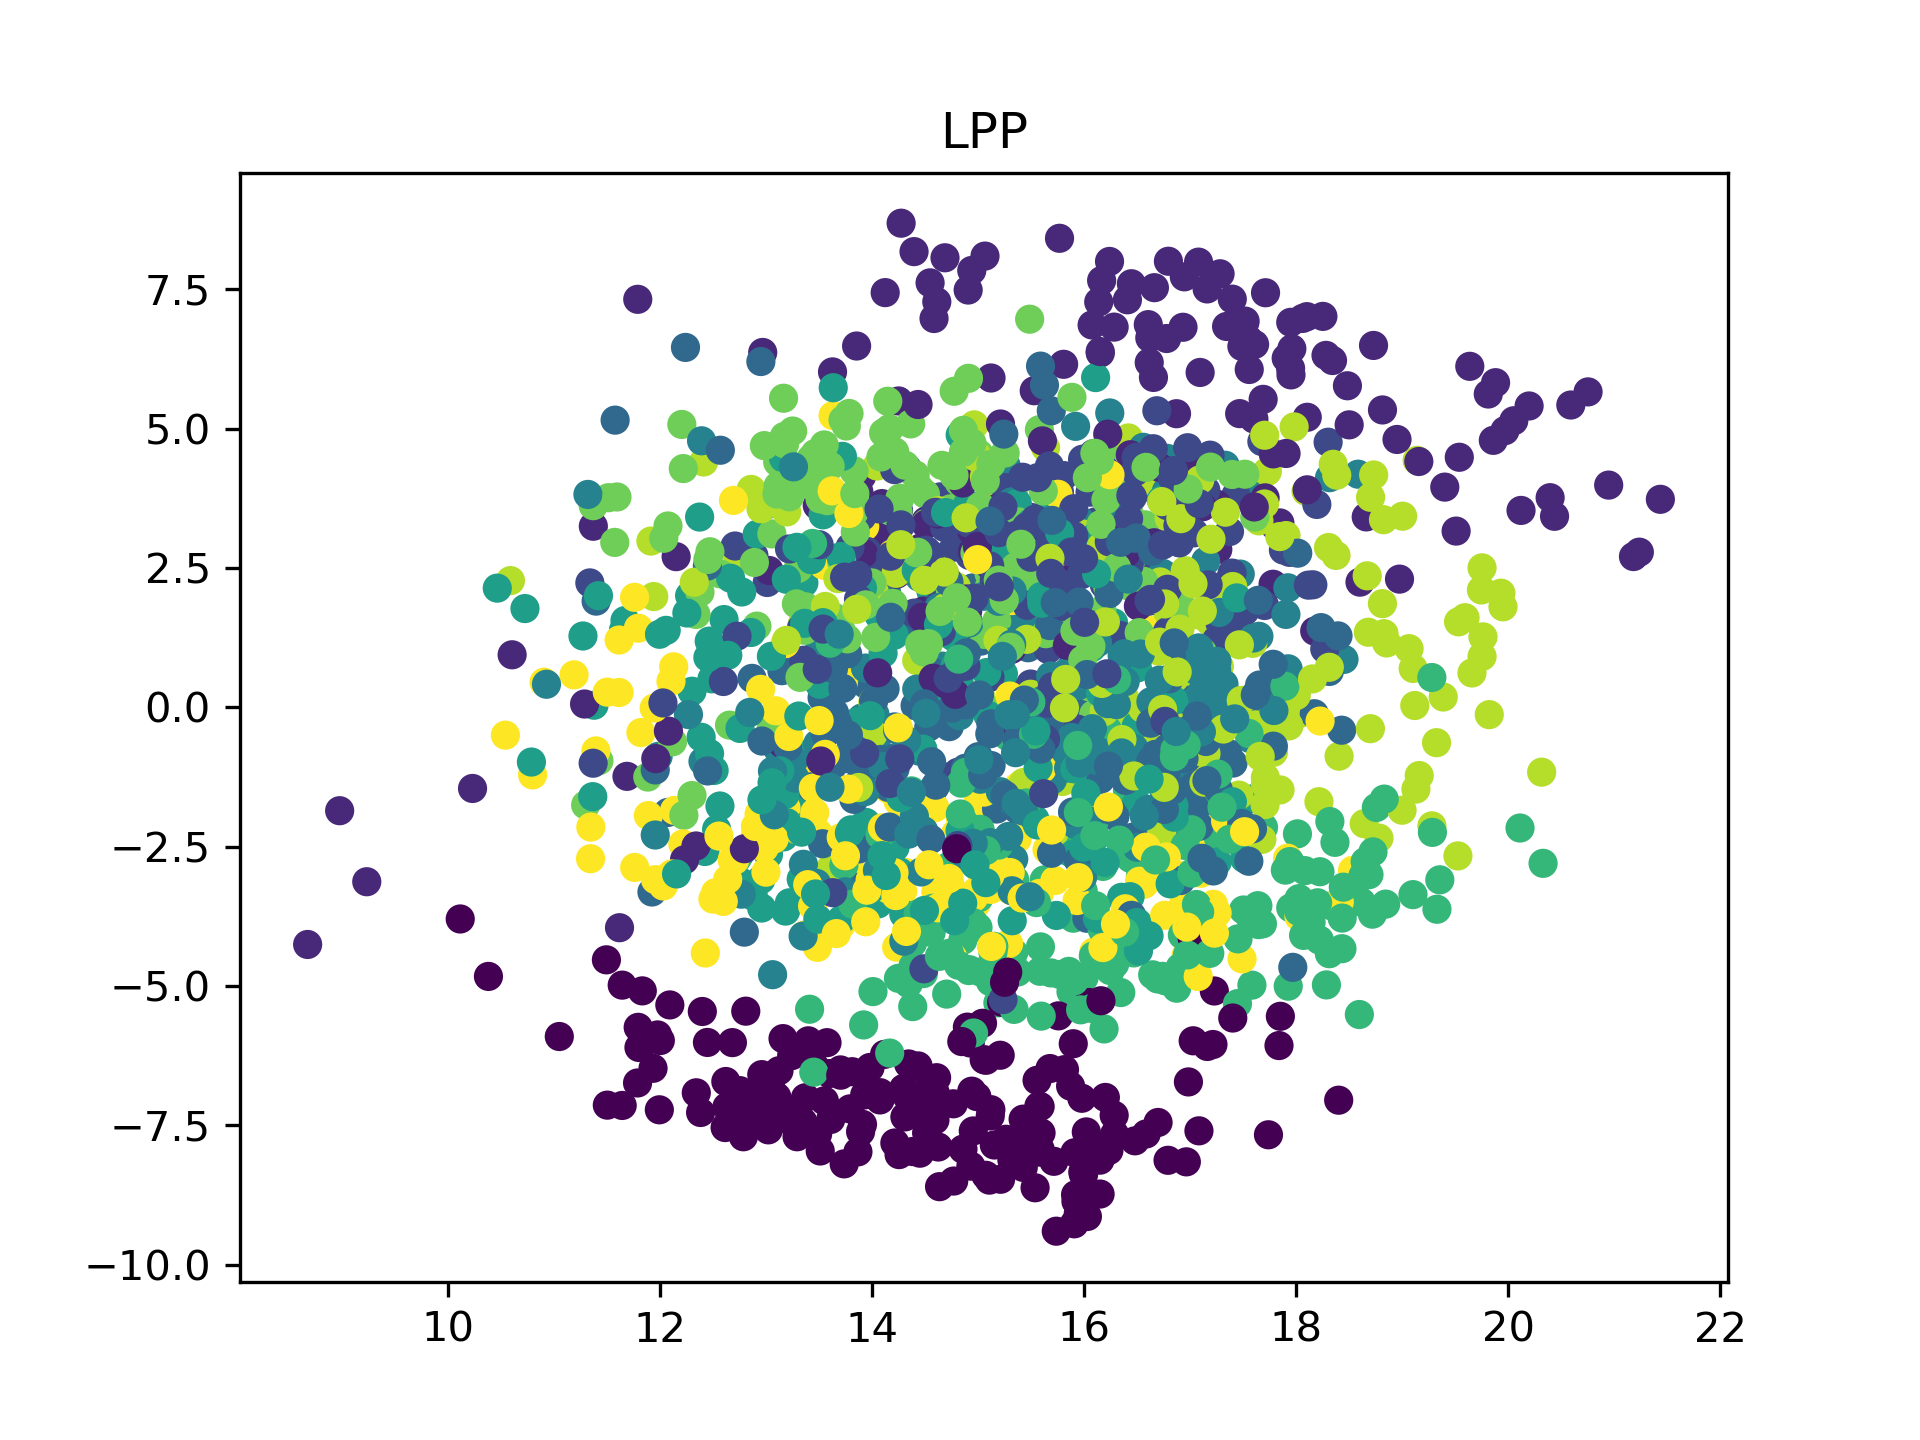
\includegraphics[width = 0.6\textwidth]{Part4/4-4.png}
                \caption{可视化}
            \end{figure}

\end{document}


